\begin{figure}[h!]
\begin{center}
\includegraphics[width = 0.5 \textwidth]{figures/data.pdf}
\caption{Observational data. 
Top: The calibrated spectrum for \excluster.
Middle: The signal-to-noise ratio.
Bottom: The spectrophotometric calibration vector determined by
\citet{schiavon05}. Note the wiggles in the calibration vector\label{fig:ggc_data}}
\end{center}
\end{figure}

\begin{figure}[h!]
%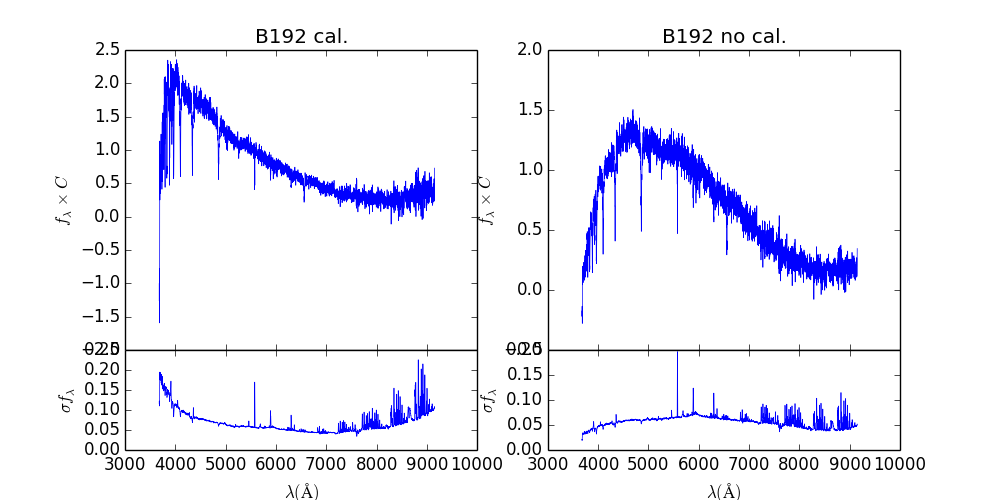
\includegraphics[width = 0.5 \textwidth]{figures/dfig_b192-g242_020.png}
\caption{A mock spectrum for a star cluster with the fiducial
parameters $10^5 M_\odot$ total stellar mass, an age of 9 Gyr, solar
metallicity, and $A_V=0.5$ mag. \label{fig:mock_data}}
\end{figure}


\begin{figure*}[h!]
\includegraphics[width=\textwidth]{figures/ideal.pdf}
\caption{Results of inference from a mock spectrum and a single
  photometric data point where the spectrophotometric calibration is
  assumed to be perfectly known. 
Top Left: The mock observed spectrum ({\it black}) is shown as well as
YY model spectra constructed from draws from the posterior PDFs of the
model parameters.
Bottom Right: Marginalized posterior PDFs for several of the physical
parameters of interest.  The input mock parameters are shown as
vertical black lines.
{\color{red} Remove calibration plot and intrinsic plot, since it is
  the same as observed spectrum.  Show residuals.}
\label{fig:speconly_ideal}}
\end{figure*}


\begin{figure*}[h!]
\includegraphics[width=\textwidth]{figures/speconly_calibrated.pdf}
\caption{Results of inference from a \emph{perfectly calibrated} mock
  spectrum and a single photometric data point, where uncertainties in
  the calibration are modeled.
Top Left: The mock observed spectrum ({\it black}) is shown as well as
YY model spectra constructed from draws from the posterior PDFs of the
model parameters, including calibration parameters {\it green}.
Bottom Left: In this case the true calibration vector ({\it black}) is a constant.
Posterior samples of the inferred calibration vector ({\it green}) include both
the polynomial and the Gaussian Process mean prediction (Equation
\ref{eq:calibration}).
Top Right: Samples of the posterior prediction for the
\emph{intrinsic} spectrum ({\it green}) as well as for the photometry
({\it magenta}).  The true mock photometry is also shown ({\it
black}).
Bottom Right: Marginalized posterior PDFs for several of the physical
parameters of interest.  The input mock parameters are shown as
vertical lines.
 {\color{red} This is not converged.  mass and dust2 PDFs will become
   much broader.}
\label{fig:speconly_calibrated}}
\end{figure*}

\begin{figure*}[h!]
\includegraphics[width=\textwidth]{figures/speconly_uncalibrated.pdf}
\caption{Results of inference from an \emph{uncalibrated} mock
  spectrum and a single photometric data point.  Panels and colors are
  as in Figure \ref{fig:speconly_calibrated}.  In this case the
  observed spectrum is in arbitrary units and the true
  calibration vector is not a constant with wavelength.
\label{fig:speconly_uncalibrated}}
\end{figure*}

\begin{figure*}[h!]
\includegraphics[width=0.5 \textwidth]{figures/photonly.pdf}
\caption{Results of inference from the photometric data only.  The
  redshift is fixed {\color{blue} (should just use a tight prior)} and
 spectroscopic calibration parameters are not modeled.
Top: The intrinsic spectrum. Samples of the posterior prediction
for the \emph{intrinsic} spectrum ({\it green}) and the
photometry ({\it magenta}).  The mock photometry is also shown
({\it black}).
Right: Marginalized posterior PDFs for several of the physical
parameters of interest.  The input mock parameters are shown as
vertical lines.
\label{fig:photonly}}
\end{figure*}

\begin{figure*}[h!]
\includegraphics[width=\textwidth]{figures/specphot_uncalibrated.pdf}
\caption{Results of inference from the combination of
  \emph{uncalibrated} spectroscopy and all the photometric data
  points.  Panels and colors are as in Figure \ref{fig:speconly_calibrated}.
\label{fig:specphot_uncalibrated}}
\end{figure*}


\begin{figure*}[h!]
\includegraphics[width=\textwidth]{figures/combined_post.pdf}
\caption{Joint posterior PDFs for several physical parameters. The
posteriors obtained from photometry only are in {\it red}, from
\emph{uncalibrated} spectroscopy and a single photometric point in
{\it blue}, and from the photometry and spectroscopy combined in {\it
magenta}.  The contours are 1 and 2-sigma contours. The true values
are indicated by {\it black points}.
\label{fig:combined_posterior}}
\end{figure*}


\begin{figure*}[h!]
%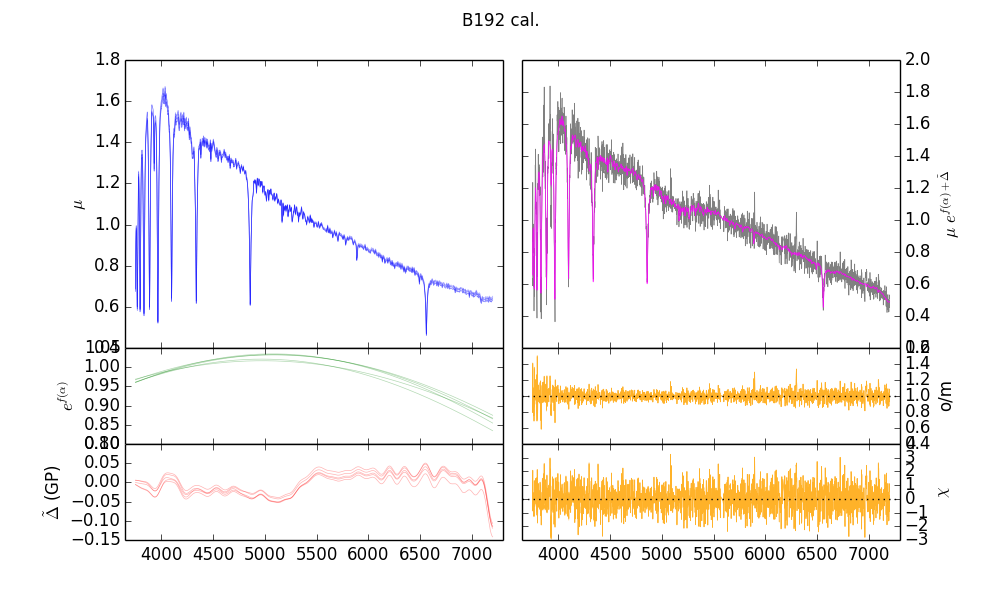
\includegraphics[width=\textwidth]{figures/sfig_b192-g242_225_cal.png}
\caption{Posterior PDFs obtained from multiple noise realizations of the
  mock photometry and uncalibrated spectra, for a single set of
  parameters.  The input mock parameters are shown as a 
  vertical line, medians of the posterior CDF for each realization are
  shown as dotted lines.
\label{fig:noise_realizations}}
\end{figure*}


\begin{figure*}[h!]
%\includegraphics[width=\textwidth]{figures/vary_params.pdf}
\caption{Offset from the input parameters of the medians of the
posterior PDFs for model parameters obtained from mock spectra and
photometry. Lines connect a single model.
 \label{fig:mock_parameter_space}}
\end{figure*}


\begin{figure*}[h!]
%\includegraphics[width=\textwidth]{figures/vary_nphot.png}
\caption{The value of more photometry. Marginalized posterior PDFs
obtained from mock spectra and photometry, for different numbers of
photometric bands.  The pdfs $g$-band only ({\it red}), $g$- and $i-$
band ({\it blue}), and the combined SDSS $griz$ and 2MASS $JHK_s$ set of
bands ({\it orange}).
\label{fig:vary_phot}}
\end{figure*}


\begin{figure*}[h!]
%\includegraphics[width=\textwidth]{figures/vary_nphot.png}
\caption{Inference from a real, calibrated, spectrum.  Top left:
  Observed spectrum and posterior samples thereof.  Bottom left:
  residuals.  Top right: inferred calibration vector, samples.
  Bottom right: posterior PDFs (corner plot?) for physical parameters.
\label{fig:real_calibrated}}
\end{figure*}

\begin{figure*}[h!]
%\includegraphics[width=\textwidth]{figures/vary_nphot.png}
\caption{Inference from a real, uncalibrated, spectrum.  Top left:
  Observed spectrum and posterior samples thereof.  Bottom left:
  residuals.  Top right: inferred calibration vector, samples.
  Bottom right: posterior PDFs (corner plot?) for physical parameters.
\label{fig:real_uncalibrated}}
\end{figure*}

\begin{figure*}[h!]
%\includegraphics[width=\textwidth]{figures/vary_nphot.png}
\caption{Ratio of the calibration vector inferred from the
  real uncalibrated spectrum to that inferred from the real calibrated
  spectrum ({\it green}). Taking the ratio reduces the effects of model
  imperfections and shows how well we are able to infer the
  calibration vector of \citet{schiavon05} ({\it black}).  
\label{fig:real_calibration_ratio}}
\end{figure*}


\begin{figure*}[h!]
%\includegraphics[width=\textwidth]{figures/vary_nphot.png}
\caption{Inferred parameters for \excluster.  We show the inference from the
  calibrated spectrum ({\it red}), from the uncalibrated spectrum
  ({\it blue}), and from the CMD ({\it black}).
\label{fig:real_parameters}}
\end{figure*}


